\section{Model-Based Reinforcement Learning (MBRL)}
All the algorithms we have looked at so far were either model-free, meaning that we 
had no model of the world and just learned value functions by interacting with the 
environment, or the dynamic programming approach, which assumes that we do have a 
model and can solve for the optimal solution without having to interact with the world. \newline
In model based reinforcement learning we learn a model from experience and use the 
learned model to do planning. By model we mean the transition probabilities/ dynamics. 
One way to learn the dynamics is to use equations of motion and then 
identify the parameters from the given data but this is not really scalable for 
complex systems. The more common approach is to use neural networks to learn the 
dynamics models. The most basic model based reinforcement learning 
algorithm would look like algorithm \ref{mbrl} where we use the experience $\{S_1,A_1,\dots,S_T\}$ 
and reduce it to a supervised learning problem.
\begin{algorithm}[H]
  \large
    \caption{Basic Model-Based RL}\label{mbrl}
    \begin{algorithmic}
        \FOR{$i=1,2,\dots$}
        \STATE collect data under the current policy
        \STATE learn dynamics model from past data
        \STATE improve policy by using dynamics model
        \ENDFOR
    \end{algorithmic}
\end{algorithm}
Model-based reinforcement learning (MBRL) offers several advantages, such as data 
efficiency, improved safety through simulation, and faster adaptation capabilities. 
However, the simple MBRL algorithm described in algortihm \ref{mbrl} also has some 
drawbacks. The problem arises from the circular dependency between data 
collection, model learning, and policy improvement. If any of these components perform 
poorly, everything can start to fail. This also introduces now two sources of approximation error: one 
from learning the model itself, and the other from using the learned model to derive the 
value function. There are many potential reasons for failure in any 
of these areas, but for now, we are focusing on the model learning aspect.

\subsection{Distributional shift}
One reason for bad performing policies which got trained by a learned model is 
distributional shift. Suppose we have trained a model on a given dataset of trajectories 
until it achieves low error on this data. However, since our model is not perfect, it will 
likely make small deviations from the true actions (e.g., slightly steering left) during 
testing. These errors accumulate over time, causing the model to encounter states it 
rarely or never saw during training. As a result, the model performs poorly on these 
unseen states.\newline
The core problem is that the state distribution on which the model was trained differs from the distribution the model generates 
during testing. Consequently, the model struggles to extrapolate to these new regions of the state space. One way to address this 
is by augmenting the training dataset with real dynamics tuples $(s,a,s')$ collected by executing the model’s own actions in the 
actual environment. This approach, which we will also revisit in the Imitation Learning chapter, helps the model adapt to the 
distribution it will face at test time.

\subsection{Model Exploitation}
The second challenge is model exploitation, a phenomenon related to overfitting, as depicted in Figure~\ref{model_exploit}. In 
this figure, the green curve represents the true Q-values, while the red curve shows the Q-values induced by the learned dynamics 
model. Since the model is used to calculate these Q-values, any inaccuracies in the model can lead to erroneous spikes in the 
predicted values. The policy, relying on these faulty predictions, may exploit these artifacts—choosing actions that appear 
optimal based on the model but are actually suboptimal or even harmful in the real environment. This can result in the policy 
overfitting to the inaccurate dynamics model (choosing this faulty spikes), leading the agent to take unrealistic actions and 
explore areas of the state space it has never encountered, ultimately causing a distributional shift.

\begin{figure}[H]
    \centering
    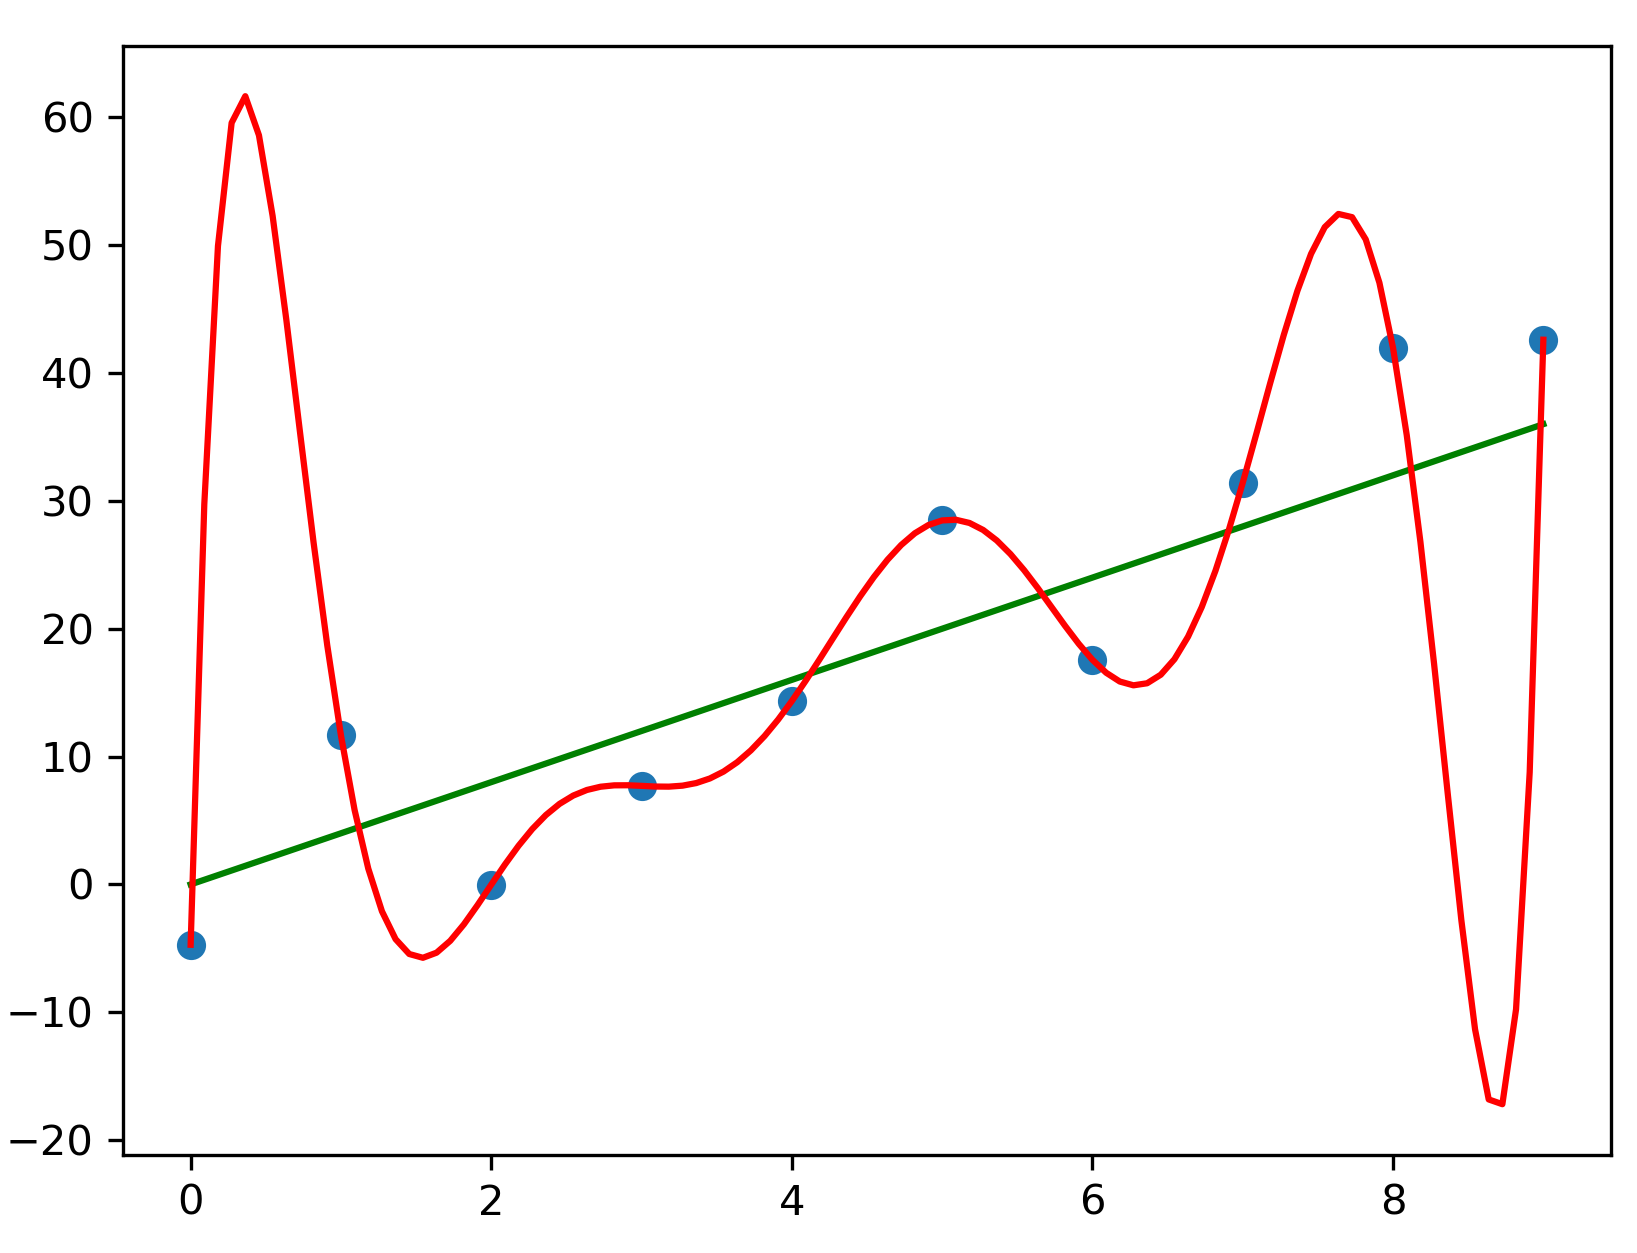
\includegraphics[width=0.5\linewidth]{images/Pyplot_overfitting.png}
  \caption{Illustration of overfitting: The green curve represents the true underlying function (ground truth), while the blue 
    dots are noisy samples drawn from it. The red curve shows the model's learned approximation, which fits the training data 
    closely but fails to generalize well. From \cite{wiki:xxx}.}
    \label{model_exploit}
\end{figure}

\subsection{Uncertainty}
One way to mitigate model exploitation is by incorporating uncertainty into the dynamics model. Rather than predicting a single 
next state for a given state-action pair, the model instead returns a distribution over possible next states. This allows the 
agent to evaluate actions based on their expected rewards while taking the uncertainty in the dynamics into account. By 
considering the full distribution of possible outcomes, the agent becomes less likely to overfit to inaccurate model predictions 
and is encouraged to choose actions that are more robust to uncertainty in the environment.
\begin{figure}[H]
    \centering
    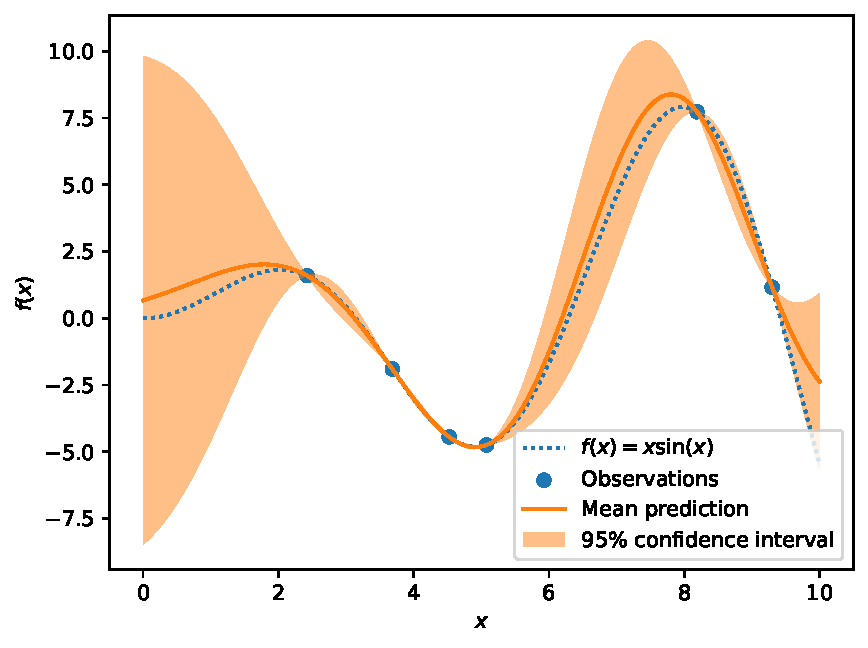
\includegraphics[width=0.7\linewidth]{images/gp_visual.pdf}
    \caption{ Gaussian process regression on noise-free dataset from \cite{GP}}
    \label{uncert_plot}
\end{figure}
However, there are several challenges with this approach. From earlier chapters, we know 
that exploration is crucial for discovering optimal policies. If our model is too 
pessimistic, it may avoid risky actions, leading to a lack of exploration. As a result, 
the agent might not discover better solutions or improve its policy. In the following 
sections, we will explore the different types of uncertainty and how we can mitigate their 
impact to encourage more effective exploration while still accounting for the uncertainty 
in the learned dynamics.

\subsubsection{Epistemic uncertainty}
Epistemic uncertainty refers to the uncertainty about the world due to a lack of 
experience (or data). This type of uncertainty can be reduced by gathering more data to 
improve our understanding. However, another approach to managing this uncertainty is to 
explicitly incorporate it into the models themselves.

\paragraph{Bayesian Learning}
Bayesian learning addresses epistemic uncertainty by treating model parameters as probabilistic rather than fixed. Instead of 
assigning a single value to each weight, we represent them as probability distributions—commonly Gaussians defined by a mean and 
variance. This probabilistic framework allows us to quantify how uncertain we are about the learned parameters. 

\paragraph{Ensembles}
Another simpler method to address epistemic uncertainty is by using an ensemble of models. 
Instead of training a single model, you train $k$ models, each of which learns the task 
independently. For prediction, we can then average the outputs of all models to obtain a 
more robust prediction.\newline
To ensure diversity among the models in the ensemble, it is helpful to train each model on 
independent training sets. This independence allows the models to explore different 
aspects of the problem and helps reduce the overall uncertainty in the predictions.

\subsubsection{ Aleatoric uncertainty}
Aleatoric uncertainty refers to the inherent uncertainty within a system, meaning that no 
matter how much experience or data you gather, some aspects will always remain uncertain. 
A classic example of aleatoric uncertainty is predicting the outcome of a dice roll. The 
outcome is uncertain, and no matter how many dice rolls you make, you can never predict 
the exact result with certainty using a deterministic function.\newline
In reinforcement learning, there are three primary sources of aleatoric uncertainty, each corresponding to a component of the Markov Decision Process (MDP):
\begin{itemize}
\item  Stochastic Rewards: When the reward function is stochastic, there is an irreducible 
uncertainty about the true value of the reward.
\item Stochastic Observations: Uncertainty in the observations received from the environment.
\item Stochastic Actions: When actions in the environment are uncertain, resulting in variability in outcomes even if the agent’s actions are deterministic.
\end{itemize}
To address aleatoric uncertainty, practitioners often use probabilistic neural networks, 
which can model this uncertainty explicitly by outputting a distribution over possible 
outcomes, rather than just point estimates. This approach allows the agent to account for 
inherent randomness in the environment and make better decisions under uncertainty.

\subsection{Replanning}
Since no learned model can perfectly predict the outcome of every action, one way to reduce the impact of model inaccuracies is 
through replanning. Unlike open-loop planning, which commits to a fixed sequence of actions and is prone to compounding errors, 
replanning continuously updates the plan based on new observations at each time step. This enables the agent to correct for past 
mistakes and adapt to changes in the environment. This strategy is commonly known as Model Predictive Control (MPC).

\subsection{Probabilistic Ensembles with Trajectory Sampling (PETS)}
PETS is a model-based reinforcement learning (MBRL) method introduced by \cite{chua2018deepreinforcementlearninghandful}. It 
represents a powerful approach to reinforcement learning by combining probabilistic modeling with planning. Rather than learning 
a policy directly, PETS simulates future outcomes using a learned model of the environment and chooses actions based on this 
simulated future.

\subsubsection{Core Components}
\begin{itemize} 
\item \textbf{Probabilistic Ensembles:}
PETS does not rely on a single neural network to model environment dynamics. Instead, it uses an ensemble of neural networks, 
each trained to predict the next state given the current state and action. These networks are probabilistic, typically outputting 
parameters of a Gaussian distribution over the next state. 

\item 
\textbf{Trajectory Sampling:}
Rather than only choosing the next action based on immediate predictions, PETS samples entire sequences of future trajectories. This is achieved by: 
\begin{itemize} 
\item Sampling multiple models from the ensemble. 
\item Simulating rollouts using these models over several timesteps. 
\item Sampling from the predicted distributions at each step (the models are probabilistic models so there outputs are 
distributions which we need to sample from in order to get the state). 
\item Evaluating the total expected reward of each trajectory. 
\end{itemize}

\item \textbf{Model Predictive Control (MPC):}
PETS uses the ensemble and trajectory sampling to perform planning at every timestep via MPC. The loop is as follows: \begin{itemize} 
\item Trajectory Sampling from the current state. 
\item Choose the sequence with the highest predicted reward. 
\item Execute only the \emph{first} action of the best sequence in the real environment. 
\item Observe the next state, update the model with new data, and repeat the process. 
\end{itemize} 
\end{itemize}

\begin{figure}[H]
    \centering
    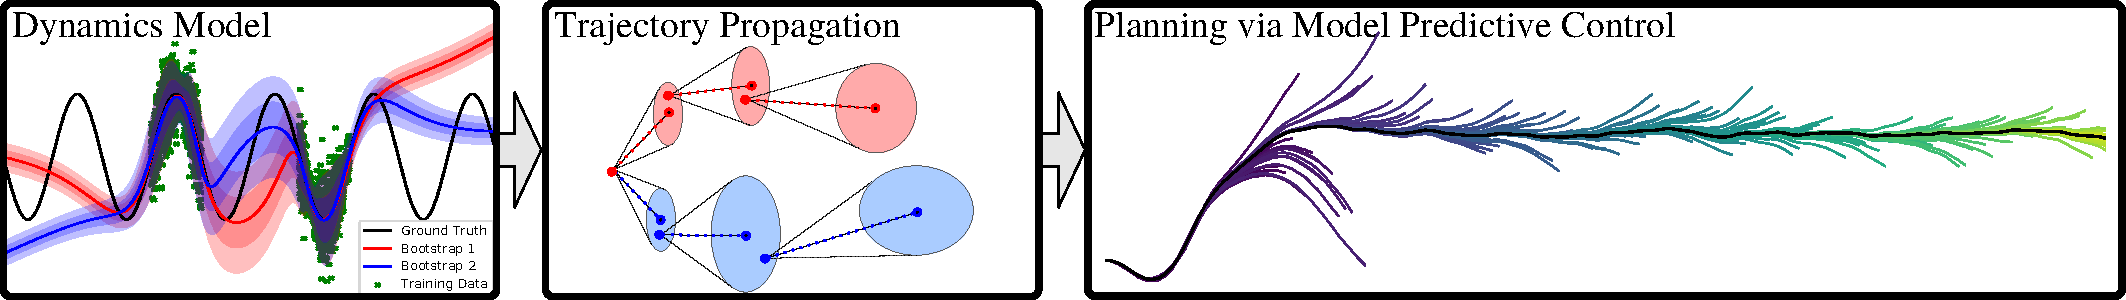
\includegraphics[width=\linewidth]{images/PETS.pdf}
    \caption{Illustration of the PETS method from \cite{chua2018deepreinforcementlearninghandful}.}
    \label{fig:PETS}
\end{figure}

\subsection{Model-Based Policy Optimization (MBPO)}
MBPO \cite{janner2021trustmodelmodelbasedpolicy} combines model-free and model-based reinforcement learning into a unified 
approach. While a dynamics model is learned from collected data, the policy is not limited to being trained exclusively in a 
model-free or model-based manner. Instead, MBPO leverages both real environment interactions and short model-generated rollouts 
to train the policy. As the agent interacts with the environment, new data is gathered to continually refine the learned model 
and improve policy performance.

\subsection{Model-Based-RL under Partial Observability}
Previous methods typically assume that environment dynamics can be represented as functions mapping state-action pairs to next 
states. However, this assumption relies on access to the true underlying states of the environment, which is often not the case 
in practice.\newline
This limitation becomes clear in image-based tasks, such as those found in Atari games. From a single image, 
it is generally impossible to directly infer latent properties like the velocity or direction of a moving object. In such cases,
the agent receives only partial observations (e.g., raw pixels), and the true state must be inferred.\newline
To address this challenge, we require a more general framework: the Partially Observable Markov Decision Process (POMDP). A POMDP 
extends the standard MDP formulation by modeling environments where the agent does not have full observability of the underlying 
state. Formally, a POMDP is defined by:

\begin{itemize}
    \item state space $S$ (not directly observable)
    \item action space $A$
    \item observation space $O$ (observable)
    \item transition model $p(s_{t+1}|s_t,a_t)$ (not known)
    \item reward function $r(s_t,a_t)$
    \item observation model $p(o_t|s_t)$
    \item initial state distribution $p(s_0)$
\end{itemize}
In general, POMDPs represent hidden Markov models, as illustrated in Figure 
\ref{pomdp_hmm}. If we knew the states $S$, the transition probabilities 
$p(s_{t+1}|s_t,a_t)$, the observation likelihoods $p(o_t|s_t)$ and if everything were 
Gaussian, we could compute the hidden states from the observations. This would allow us to 
apply the methods we've been using all along to learn policies. However, in reality, none 
of these assumptions typically hold.
\begin{figure}[H]
    \centering
\begin{tikzpicture}
\tikzset{
  main/.style={circle, minimum size = 5mm, thick, draw =black!80, node distance = 7mm},
  connect/.style={-latex, thick},
  box/.style={rectangle, draw=black!100}
}
  \node[main] (L1) [] {$S_1$};
  \node[main] (L2) [right=of L1] {$S_2$};
  \node[main] (L3) [right=of L2] {$S_3$};
 % \node[main] (Lt) [right=40mmof L3] {$S_t$};
  \node[] (Lhid) [right=7mm of L3] {$\dots$};
  
\node[main] (A1) [above = of L1] {$A_1$};
\node[main] (A2) [above = of L2] {$A_2$};
\node[main] (A3) [above = of L3] {$A_3$};
%\node[main] (At) [below left=10mm of Lt] {$A_{t-1}$};


  \node[main,fill=black!10] (O1) [below=5mmof L1] {$O_1$};
  \node[main,fill=black!10] (O2) [below=5mmof L2] {$O_2$};
  \node[main,fill=black!10] (O3) [below=5mmof L3] {$O_3$};
  %\node[main,fill=black!10] (Ot) [below=of Lt] {$O_t$};
  \path (L1) edge [connect] (L2)
        (L2) edge [connect] (L3)
        (L3) edge [connect] (Lhid);
        %(Lhid) edge [connect] (Lt);
        
  \path (A1) edge [connect] (L2)
        (A2) edge [connect] (L3)
        (A3) edge [connect] (Lhid);
        %(At) edge [connect] (Lt);
  \path (L1) edge [connect] (O1);
  \path (L2) edge [connect] (O2);
  \path (L3) edge [connect] (O3);
  %\path (Lt) edge [connect] (Ot);
\end{tikzpicture}
    \caption{A POMDP illustrated as a hidden markov chain}
    \label{pomdp_hmm}
\end{figure}
A common approach in model-based reinforcement learning under partial observability is to first learn a mapping from high-
dimensional observations (e.g., images) to a lower-dimensional latent state space. This latent space is designed to capture the 
essential features of the environment needed for decision-making, even if it does not correspond directly to the true underlying 
state. To learn this mapping, Variational Autoencoders (VAEs) are typically used, providing both an encoder (from observation to 
latent state) and a decoder (from latent state back to observation). Once this representation is learned, the dynamics model is 
trained directly in the latent space.\newline 
There are several possible choices for modeling the encoder. The most accurate approach is to learn the posterior $q_\psi(s_t 
\mid o_{1:t}, a_{1:t})$, which incorporates the full history of observations and actions. However, while this posterior provides 
the most precise estimate of the latent state, it is also the most complex to learn. A simpler, though less accurate, alternative 
is to use a single-step encoder, which learns the posterior $q_\psi(s_t \mid o_t)$ based solely on the current observation. \newline
In recent years, several methods have been proposed that excel in model-based reinforcement learning. While a detailed discussion
is beyond the scope, here are some notable approaches:
\begin{itemize} 
\item PlaNet (introduced Recurrent State Space Models (RSSM) ) \cite{hafner2019learninglatentdynamicsplanning}
\item Dreamer (Dream to Control) \cite{hafner2020dreamcontrollearningbehaviors}
\end{itemize}

\subsection{Self-Test Questions}
\begin{enumerate}
\sq{ What is the difference between model-based and model-free RL?}\newline
In model-based RL, we learn a model of the environment and use it for planning. In model-
free RL, we don't focus on learning a model; instead, we learn value functions or policies 
by directly interacting with the environment.

\sq{Why is model learning in MBRL not just supervised learning?}\newline
In supervised learning, our data comes from a single underlying distribution $p$ and we 
aim to learn the mapping from features to labels. However, model learning in model-based 
RL (MBRL) is cyclic. We use the model to improve a policy, which then generates new data 
that is used to further optimize the model. This feedback loop results in a shifting 
distribution of data, so there is no fixed objective, unlike in supervised learning.

\sq{What are the different types of uncertainty, how can they be captured and why is that important for MBRL?} \newline
There are two primary types of uncertainty:
\begin{itemize}
    \item Epistemic uncertainty: This refers to the uncertainty about the world due to a 
    lack of data. It can be reduced by gathering more data or incorporating uncertainty 
    directly into the model (e.g., through Bayesian learning).
    \item Aleatoric uncertainty: This refers to uncertainty inherent in the system, meaning no matter how much data we gather, some uncertainty remains irreducible. This type of uncertainty can be captured by using probabilistic models.
\end{itemize}
Understanding and addressing these types of uncertainty is crucial in model-based 
reinforcement learning (MBRL). If uncertainty is not properly accounted for, it can lead 
to model exploitation, where the agent might overfit to the learned model and make poor 
decisions based on inaccurate predictions, ultimately impacting the performance of the 
policy.

\sq{How can you plan with an imperfect model?}\newline
One approach is replanning after each action is taken, turning an open-loop problem into a 
closed-loop process. This way, the agent can adjust based on new observations and model 
corrections.

\sq{What is partial observability, why is it important?}\newline
Partial observability occurs when we cannot fully observe the state of the environment. In 
many real-world scenarios, this happens due to missing sensor data or limited context 
(e.g., in image-based tasks like Atari, where a single image doesn’t provide information 
about the ball's velocity or direction). Since we can't directly observe the state, this 
complicates the use of algorithms that assume full observability.

\sq{What are the state space assumptions?}
\begin{itemize}
    \item observations only depend on the current state $p(o_t|s_t)$
    \item states depend only on the previous state and the action $p(s_{t+1}|s_t,a_t)$
\end{itemize}

\sq{How can we use Variational Inference to learn deep SSMs/sequential VAEs?}\newline

\sq{How can we use those for model based RL under partial observability?}\newline
Sequential VAEs and deep state-space models encode observations into a lower-dimensional 
latent space that represents the states. This latent space can then be used by a dynamics 
or inference model to predict future states, enabling planning and decision-making despite 
partial observability.

\sq{How can you use a model to learn a parametric policy?}\newline
A parametric policy can be learned by training policy networks and value-function networks 
on imagined or simulated trajectories generated by the learned model. These simulated 
trajectories provide a way to refine the policy without needing real-world data.

\end{enumerate}

\subsection{Resources}
Much of the general content presented here is based on Sergey Levine’s CS 285: Lecture 11 \cite{CS285,CS285LevineYoutube}. A 
highly informative blog post \cite{Dreamer_V1} by one of the authors of Dreamer V1, detailing the method . I also recommend 
checking out the blog post by Danijar Hafner \cite{danjar}, one of the key contributors behind many of the world models papers.
